%%%%%%%%%%%%%%%%%%%%%%%%%%%%%%%%%%%%%%%%%%%%%%%%%%%%%%%%%%%%%%%%%
% Contents: The QIF chapter
% $Id: grisbi-manuel-QIF.tex, v 0.4 2002/10/27 Daniel Cartron
% $Id: grisbi-manuel-QIF.tex, v 0.5.0 2004/06/01 Loic Breilloux
% $Id: grisbi-manuel-QIF.tex, v 0.6.0 2011/11/17 Jean-Luc Duflot
% $Id: grisbi-manuel-QIF.tex, v 0.8.9 2012/04/27 Jean-Luc Duflot
% $Id: grisbi-manuel-QIF.tex, v 1.0 2014/02/12 Jean-Luc Duflot
%%%%%%%%%%%%%%%%%%%%%%%%%%%%%%%%%%%%%%%%%%%%%%%%%%%%%%%%%%%%%%%%%


\chapter{Export et import de comptes\label{move}}

Vous ne pouvez pas utiliser directement dans Grisbi des données qui ont été créées par d'autres applications de comptabilité personnelle, et réciproquement. Comme ces applications fonctionnent différemment, leurs données sont structurées différemment: il faut donc convertir leur structure de données avant de pouvoir les utiliser. 

Cette conversion ne peut pas se faire d'un seul coup sur l'ensemble des données, mais doit se faire indépendamment pour chaque compte géré par l'application. Pour convertir chacun de ces comptes, il faut donc d'une part les \og exporter \fg{} de l'application d'origine, puis les \og importer \fg{} dans l'application de destination.

% espace avant Attention ou Note  : 5 mm
\vspacepdf{5mm}

\strong{Attention} : ne pas confondre LE \og fichier de comptes \fg{} qui contient toutes les données de tous les comptes créés pour la gestion d'une entité comptable (dans Grisbi, ce fichier porte l'\gls{extension} \file{.gsb}), et LES \og fichiers de compte \fg{}, qui sont des fichiers ne contenant que les données d'un seul compte à la fois, et créés uniquement pour exporter ou importer ces données d'une application de comptabilité à une autre. Ces \og fichiers de compte \fg{} doivent avoir un \gls{format de fichier} (ou une extension) obligatoirement compatible avec l'application d'origine ET l'application de destination.
% espace après Attention ou Note  : 5 mm
\vspacepdf{5mm}

Grisbi supporte actuellement les formats de données de compte de comptabilité personnelle \gls{Gnucash}, \gls{OFX}, \gls{CSV} et \gls{QIF}.


\section{Import de comptes d'un autre logiciel\label{move-import}}


Si vous voulez utiliser dans Grisbi des données de comptes qui ont été créés
dans une autre application de comptabilité, vous devez d'abord exporter individuellement chacun des comptes de cette application dans un fichier, puis les importer dans Grisbi grâce à ces fichiers.


\subsection{Export d'un fichier de compte d'un autre logiciel\label{move-import-exportinit}}

La première étape consiste, dans l'application de comptabilité personnelle
d'origine, à exporter chaque compte dans un fichier au format choisi. Le format choisi doit être compatible à l'exportation par l'application d'origine \emph{et} compatible à l'importation par Grisbi.

La procédure d'exportation est bien évidemment différente pour chaque logiciel, donc référez-vous à sa documentation. Si vous voulez exporter tous les comptes, vous devrez obtenir autant de fichiers que vous avez de comptes gérés par l'application.


\subsection{Import de fichiers de compte d'un autre logiciel dans Grisbi\label{move-import-importinit}}

\textbf{Note} : Grisbi permet d'importer un ou plusieurs fichiers de compte au cours de la même procédure. Bien que l'on puisse importer les fichiers de compte un par un, il est important de bien importer tous les fichiers de compte simultanément, afin que Grisbi puisse recréer les liens entre les comptes, particulièrement en ce qui concerne les opérations de virement.
% espace après Attention ou Note  : 5 mm
\vspacepdf{5mm}

Pour plus de renseignements sur les \indexword{types de compte}\index{types de compte} que Grisbi sait gérer,  voir la section \vref{accounts-type}, \menu{Types de comptes de Grisbi}.

Vous pouvez définir quelle date sera utilisée pour l'attribution d'un exercice à 
chaque opération importée, voir le paragraphe \vref{setup-general-import-financialyear}, \menu{Définition de l'exercice}.

Lorsque vous importez un fichier, Grisbi vous permet d'établir une association entre une chaîne de caractères de ce fichier et un tiers. Par exemple, tous les libellés contenant \og loyer \fg{} peuvent être associés à un tiers qui représente votre propriétaire. Cela doit être configuré dans le menu \menu{Édition - Préférences} (voir la section \vref{setup-general-importLinks}, \menu{Associations pour l'import}).

% espace pour changement de thème
\vspacepdf{5mm}
Dans le menu \menu{Fichier} de Grisbi, choisissez l'option \menu{Importer un
fichier}, ce qui ouvre la fenêtre de l'assistant d'importation. L'importation des fichiers de compte se déroule en cinq étapes :

\begin{enumerate}
	\item accueil de l'assistant d'importation ; validez par le bouton \menu{Suivant} ;
	\item sélection des fichiers de compte à importer :	
		\begin{enumerate}
			\item cliquez sur le bouton \menu{Ajouter un ou des fichiers} : une fenêtre de gestionnaire de fichiers s'ouvre,	
			\item cherchez le répertoire où se trouvent ces fichiers de compte,
			\item sélectionnez un ou plusieurs fichiers de compte (avec la combinaison  \key{Ctrl}\key{Clic} et \key{Majuscule}\key{Clic}) ; vous pouvez aussi changer la \gls{locale} (\gls{encodage des caracteres}) des fichiers à importer dans le menu déroulant \menu{Codage},
			\item validez la fenêtre pour revenir à la fenêtre de sélection des fichiers de compte,
			\item si les sélections voulues sont bien cochées, vous pouvez valider par le bouton \menu{Suivant} ;
		\end{enumerate}		  
	\item fin de la préparation de l'importation des fichiers de compte : si tout s'est bien passé, cette fenêtre donne la liste des fichiers de compte qui seront importés ; continuez l'importation en validant par le bouton \menu{Suivant} ;
	\item création et paramétrage de chaque compte importé dans Grisbi : vous pouvez passer en revue chaque compte et y choisir les actions suivantes \ifIllustration \refimage{QIF-import-files-setup-img} :
	% image centrée
	\begin{figure}[htbp]
	\begin{center}
	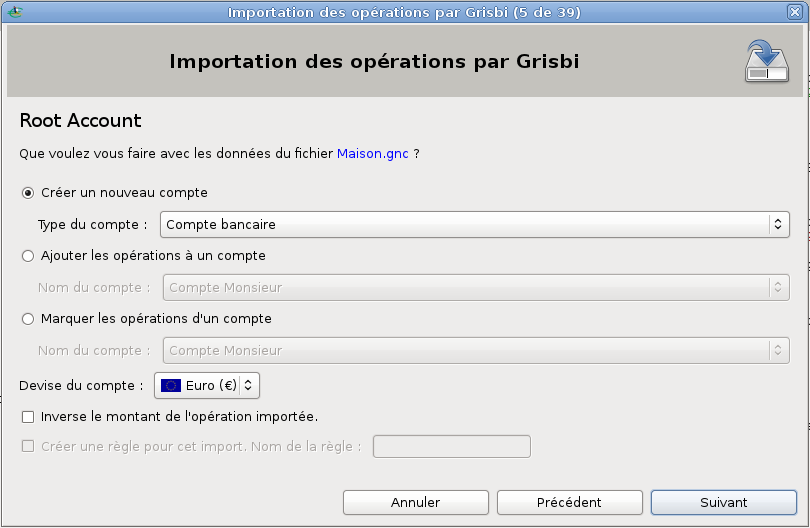
\includegraphics[scale=0.5]{image/screenshot/QIF_import_files_setup}
	\end{center}
	\caption{Paramétrage de chaque compte importé}
	\label{QIF-import-files-setup-img}
	\end{figure}
	% image centrée
	\else  :
	\fi
	
		\begin{itemize}
			\item créer un nouveau compte,
			\item ajouter des opérations à un compte : si des opérations planifiées sont trouvées dans l'intervalle de temps spécifié, une fenêtre spécifique s'ouvre pour savoir ce que vous voulez en faire : soit fusionner ces opérations planifiées avec les opérations importées correspondantes, soit ajouter les opérations importées en sus de celles-là (voir la section \vref{setup-general-import-parameters}, \menu{Paramètres pour l'import}),
			\item marquer les opérations d'un compte : si des \indexword{opérations orphelines}\index{opération !orpheline} sont trouvées, une fenêtre s'ouvrira en fin d'import pour savoir ce que vous voulez en faire : soit les ajouter, soit les ignorer,
			\item définir la devise du compte (ou bien en créer une nouvelle),
			\item   inverser le montant de l'opération (utile pour les comptes de carte bancaire de la Banque Postale, par exemple),
			\item créer une règle d'importation rapide si le fichier est au format QIF ou OFX,
			\item quand tout est correct, validez l'importation par le bouton \menu{Suivant} ;
		\end{itemize}
	
	 \item validation de la fin de l'importation : valider par le bouton \menu{Fermer}.
\end{enumerate}

Si, et seulement si vous venez de créer votre fichier de comptes juste avant cette importation de données de comptes, revenez à la fin de la section \vref{start-newfile-end}, \menu{Création d'un nouveau fichier de comptes}. Allez juste après la fin de la procédure de création du fichier de comptes, au paragraphe commençant par \emph{D'une manière ou d'une autre\ldots{ }}, ce qui vous proposera de créer tout de suite d'autres comptes.

%espace pour changement de thème
\vspacepdf{5mm}
Sinon, vous pouvez commencer à utiliser le compte que vous venez de créer.


\section{Export de comptes à partir de Grisbi\label{move-export}}


Si vous voulez utiliser, dans une autre application de comptabilité, des données de compte qui ont été créées par Grisbi, vous devez d'abord exporter ces données dans des fichiers, puis les importer dans l'autre application grâce à ces fichiers. Le format de fichier choisi doit être compatible à l'exportation par Grisbi \emph{et} compatible à l'importation par l'application de destination.
 
Dans le menu \menu{Fichier} choisissez l'option \menu{Exporter vers un fichier QIF/CSV/\ldots{ }} qui ouvre l'assistant Export des comptes. L'exportation des comptes comporte quatre étapes :

\begin{enumerate}
	\item accueil de l'assistant ; cette fenêtre indique que, comme les formats de fichier QIF et CSV ne supportent pas les devises, toutes les opérations seront converties dans la devise de leur compte respectif ; validez par le bouton \menu{Suivant} ;
	\item sélectionnez les comptes à exporter en cliquant dans la case correspondante ; validez par le bouton \menu{Suivant} ;
	\item pour chaque compte, définissez le nom du fichier, le répertoire de destination et le format d'exportation, puis validez par le bouton \menu{Suivant} \ifIllustration \refimage{QIF-export-img} ;
	% image centrée
	\begin{figure}[t]
	\begin{center}
	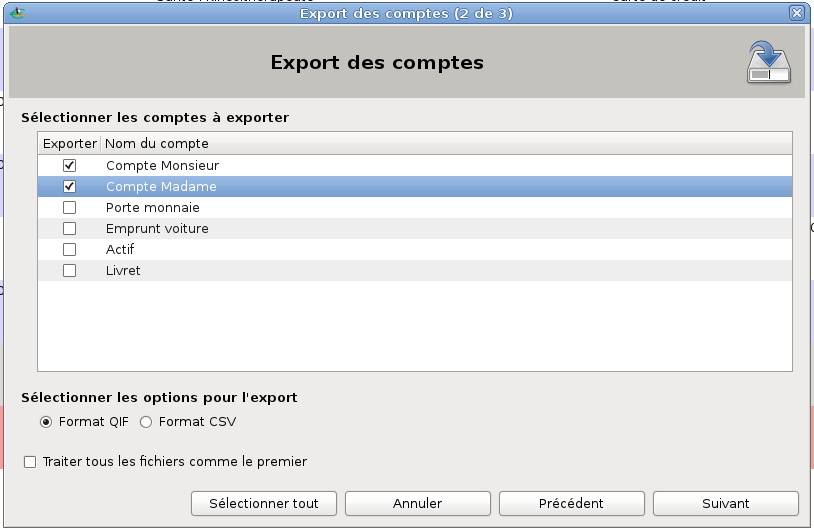
\includegraphics[scale=0.5]{image/screenshot/QIF_export}
	\end{center}
	\caption{Export des comptes}
	\label{QIF-export-img}
	\end{figure}
	% image centrée
	\else  ;
	\fi
	
	\item la fenêtre de fin de l'exportation s'affiche ; validez par le bouton \menu{Fermer}.
\end{enumerate}

\strong{Attention} : d'une manière générale, il est déconseillé d'avoir des accents ou des espaces dans les noms des répertoires et fichiers utilisés par Grisbi. Si c'est le cas, renommez-les maintenant. Par exemple, les espaces peuvent être remplacées par des tirets bas (\_).











